\documentclass[a4paper]{article}
\usepackage[utf8]{inputenc}
\usepackage[russian]{babel}
\usepackage[T2]{fontenc}
\usepackage[warn]{mathtext}
\usepackage{graphicx}
\usepackage{amsmath}
\usepackage{floatflt}
\usepackage[left=20mm, top=20mm, right=20mm, bottom=20mm, footskip=10mm]{geometry}


\graphicspath{ {images/} }
\usepackage{multicol}
\setlength{\columnsep}{2cm}


\begin{document}

\begin{titlepage}
	\centering
	\vspace{5cm}
	{\scshape\LARGE Московский физико-технический институт \par}
	\vspace{4cm}
	{\scshape\Large Лабораторная работа \par}
	\vspace{1cm}
	{\huge\bfseries Интерференция электромагнитных волн милиметрового диапазона \par}
	\vspace{1cm}
	\vfill
\begin{flushright}
	{\large выполнила студентка 653 группы ФФКЭ}\par
	\vspace{0.3cm}
	{\LARGE Карпова Татьяна} \par

\end{flushright}
	

	\vfill

% Bottom of the page
	Долгопрудный, 2018 г.
\end{titlepage}

\section{Цель работы}
Изучение интерференции электромагнитных волн миллиметрового диапазона с применением двух оптических интерференционных схем, экспериментальное определение длины волны излучения и показателя преломления диэлектрика

\section{В работе используются:}
\begin{itemize}
    \item приёмно-передающая система радиоволн миллиметрового диапазона
    \item металлические зеркала
    \item микрометрический винт
    \item проволочная решётка
    \item пластина из диэлектрика
\end{itemize}

\section{Теоретические положения}
Если в некоторой точке пространства происходит суперпозиция двух когерентных одинаково поляризованных волн с интенсивностями $I_1$ и $I_2$ и с разностью фаз $\varphi$, то интенсивность $I$ результирующего колебания определяется соотношением 
\begin{equation}
    I = I_1 + I_2 + 2\sqrt{I_1 I_2}\cos \varphi
\end{equation}
Интенсивность максимальна при $\varphi = 2\pi m$, минимальна при $\varphi = (2m+1)\pi$ ($m = 0, 1, 2, ...$ - порядок интерференции)

\section{Экспериментальная установка}
Источником миллиметровых волн является генератор на клистроне — специальной лампе, генерирующей сверхвысокочастотные колебания. Из клистрона энергия волны подается в прямоугольный волновод. Волноводом называется полая металлическая труба, используемая в СВЧ-диапазоне волн для передачи энергии. Клистрон возбуждает в волноводе
электромагнитную волну, которая распространяется вдоль волновода и с помощью рупорной антенны излучается в пространство. Задача антенны заключается в том, чтобы сделать излучение более направленным. Направленность антенны характеризуют шириной её диаграммы направленности. Чем шире раскрыв рупорной
антенны, тем уже ее диаграмма направленности. \par
Отражённое от препятствия электромагнитное излучение, попадая в рупорную антенну приемника, распространяется по волноводу, в котором имеется детектор высокочастотных колебаний,
работающий в квадратичном режиме. Поэтому ток детектора пропорционален интенсивности I волны, попадающей в приемную антенну. Сигнал с выхода детектора усиливается и измеряется микровольтметром. Принципиальная схема приёмно-передающего тракта представлена на рис. 1.

\begin{figure}[h]
    \centering
    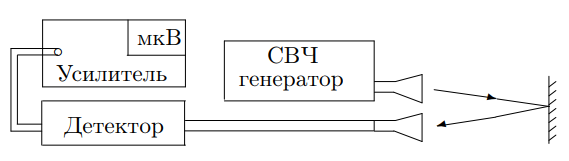
\includegraphics[width=12cm]{fig1.PNG}
    \caption{Приёмно-передающая система СВЧ-диапазона}
    \label{fig:vac}
\end{figure}

Применяемый в настоящей работе передатчик излучает линейно поляризованную волну, электрический вектор \textbf{E} которой перпендикулярен широкой стенке волновода. Приемник также может принимать только линейно поляризованную волну. Для установления связи в системе, изображенной на рис. 1, необходимо, чтобы широкие стенки волноводов передатчика и приемника были параллельны друг другу.
Если одну из антенн повернуть относительно луча на некоторый угол $\alpha$, интенсивность принимаемого сигнала будет изменяться по \textit{закону Малюса}
\begin{equation}
    I = I_0 \cos^2 \alpha
\end{equation}

\subsection{Интерференция радиоволн, отражённых от зеркала и решётки}
Схема установки, используемой для этого опыта, приведена на рис. 2. \par
Металлическое зеркало З и проволочная решетка Р устанавливаются на некотором расстоянии d
друг от друга с помощью специальных фиксаторов. Приемная и передающая антенны располагаются
симметрично, так чтобы в приемник попадала отраженная волна.
Волна, излучаемая передающей антенной, частично отражается от решетки, а частично проходит через нее и отражается от зеркала. Зеркало может перемещаться при помощи микрометрического винта. \par 
Между волнами, отраженными от решетки и от зеркала, возникает разность хода, равная
\begin{equation}
    \triangle = 2 d \cos \theta.
\end{equation}
При изменении разности хода (при изменении d) интенсивность волны в точке приема изменяется в соответствии с формулой (1)

\subsection{Интерферометр Майкельсона}
В этом опыте используется установка, моделирующая оптический интерферометр Майкельсона (рис. 3). Зеркала З1 и З2 располагаются перпендикулярно осям
передающей и приемной антенн, которые в свою очередь должны быть взаимно перпендикулярны. Решетка Р располагается на пересечении осей под углом 45◦ к ним. Волна от передающей антенны
расщепляется на решетке на две волны, распространяющиеся в направлении зеркал З1 и З2. После отражения от зеркал обе волны
возвращаются к решетке. Каждая из этих волн после вторичного расщепления на решетке Р частично попадает в приемную антенну. \par

Разность хода ∆ возникает вследствие различия в расстояниях
$l_1$ и $l_2$ между решеткой Р и зеркалами З1 и З2:
\begin{equation}
    \triangle = 2 (l_2 - l_1).
\end{equation}

При изменении длины одного из плеч интерферометра (при перемещении соответствующего зеркала) интенсивность в точке
приема изменяется в соответствии с формулой (1). \par

Если на пути одного из лучей поставить пластинку толщиной $d_0$ с диэлектрической проницаемостью $\varepsilon$, разность хода изменится
на величину $2 d_0 (n−1)$, где $n = \sqrt{\varepsilon}$ —
показатель преломления вещества,
из которого сделана пластинка. Это
приводит к изменению интенсивности в точке приема. Пусть в точке приема до внесения пластинки наблюдался интерференционный максимум. Для того чтобы получить тот же максимум при наличии пластинки, нужно зеркало свободного плеча интерферометра (плеча, в котором нет пластинки) отодвинуть на расстояние $\triangle x_0$, определяемое выражением
\begin{equation}
    \triangle x_0 = d_0 (n-1).
\end{equation}
Зная $\triangle x_0$, можно определить показатель преломления.

\begin{figure}[h]
\begin{center}
\begin{minipage}[h]{0.45\linewidth}
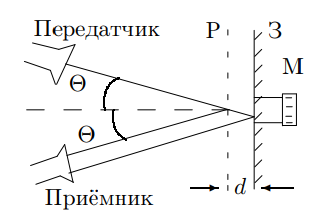
\includegraphics[width=1\linewidth]{fig2.PNG}
\caption{Интерференция волн СВЧ в плоскопараллельной пластине} %% подпись к рисунку
\label{ris:experimoriginal} %% метка рисунка для ссылки на него
\end{minipage}
\hfill 
\begin{minipage}[h]{0.45\linewidth}
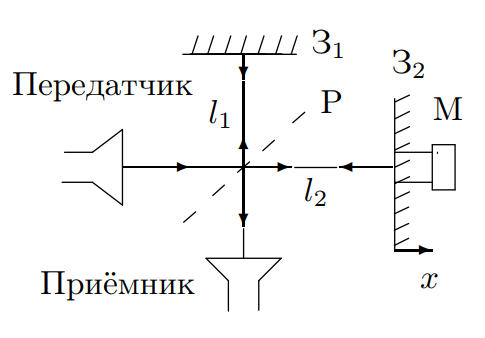
\includegraphics[width=1\linewidth]{fig3.PNG}
\caption{Интерферометр Майкельсона на СВЧ}
\label{ris:experimcoded}
\end{minipage}
\end{center}
\end{figure}

\section{Ход работы}
\subsection{Проверка закона Малюса}
\begin{enumerate}
    \item Расположим рупоры как показано на рис. 2, настроим установку на максимум интенсивности методом последовательных приближений.
    \item Снимем зависимость уровня сигнала $I$ от угла поворота $\alpha$ приёмной антенны относительно луча, убедимся, что излучаемая электромагнитная волна линейно поляризована
    \item Построим графики зависимости уровня сигнала $I$ от $\cos^2 \alpha$, убедимся в справедливости закона Малюса (2)
    
\begin{figure}[h]
\begin{center}
\begin{minipage}[h]{0.45\linewidth}
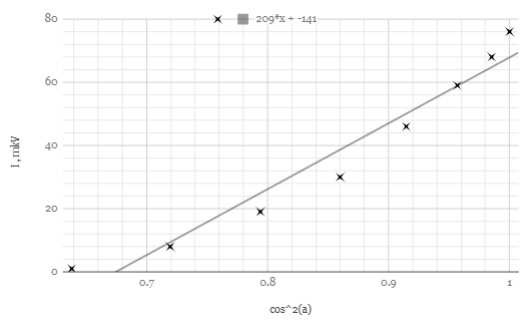
\includegraphics[width=1\linewidth]{mal1.PNG}
\caption{Зависимость $I$ от $\cos^2 \alpha$, уменьшение угла} %% подпись к рисунку
\label{ris:experimoriginal} %% метка рисунка для ссылки на него
\end{minipage}
\hfill 
\begin{minipage}[h]{0.45\linewidth}
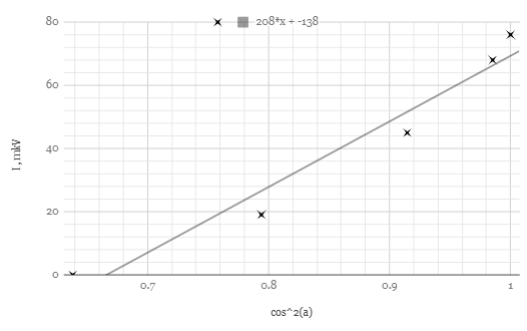
\includegraphics[width=1\linewidth]{mal2.PNG}
\caption{Зависимость $I$ от $\cos^2 \alpha$, увеличение угла}
\label{ris:experimcoded}
\end{minipage}
\end{center}
\end{figure}
\end{enumerate}

\subsection{Интерференция волн, отражённых от зеркала и решётки}
\begin{enumerate}
    \item Закрепим на фиксаторах перед зеркалом металлическую решётку, убедимся, что при перемещении зеркала уровень сигнала в точке приёма изменяется
    \item Снимем зависимость интенсивности $I$ от координаты $x$ подвижного зеркала. Построим график зависимости $I(x)$
    
\begin{figure}[h]
    \centering
    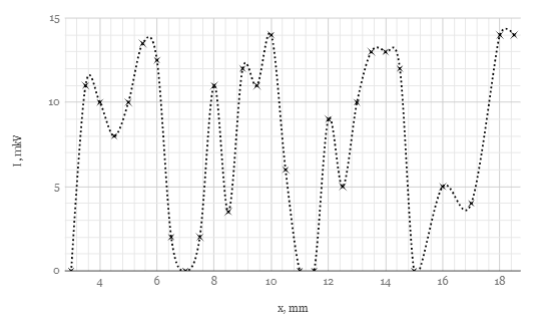
\includegraphics[width=14cm]{graph1.PNG}
    \caption{График зависимости интенсивности сигнала от координаты подвижного зеркала}
    \label{fig:vac}
\end{figure}

Длина волны, определённая по этому графику - $\lambda_1 = 8.167$ мм. \par
Длина волны по частотогенератору: $\lamda_0 = 8.333$ мм (частота 36 ГГЦ).
\end{enumerate}

\subsection{Интерферометр Майкельсона}
\begin{enumerate}
    \item Соберём схему интерферометра Майкельсона согласно рис. 3, настроим установку на максимум сигнала. 
    \item Перемещая подвижное зеркало З2, снимем зависимость координаты $x_m$ в точке интерференционного максимума от номера максимума $m$, построим график зависимости $x_m = f(m)$
    
\begin{figure}[h]
    \centering
    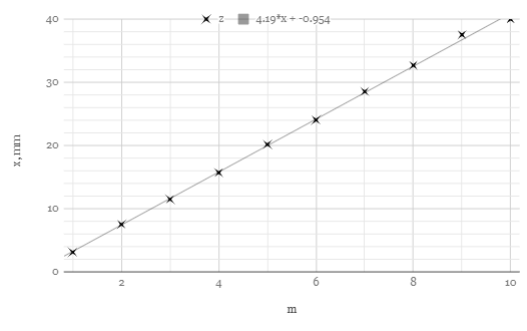
\includegraphics[width=14cm]{graph2.PNG}
    \caption{График зависимости координаты подвижного зеркала от номера интерференционного максимума}
    \label{fig:vac}
\end{figure}

По графику определим длину волны: $\lambda_2 = 8.38$ мм

\item Поместим перед подвижным зеркалом З2 тефлоновую пластину толщиной $3.25$ мм. Смещение интерференционного максимума от прежнего положения составляет $9$ мм. По формуле (5) определим показатель преломления тефлона: $n_1 = 1.36$. Табличное значение: $n_0  = 1.4$
\end{enumerate}
    
\section{Вывод}
В ходе работы была изучена интерференция электромагнитных волн миллиметрового диапазона с помощью оптических схем. Несколькими способами определена длина волны:
\begin{center}
    $\lambda_0 = 8.333$ мм (частотогенератор) \par
    $\lambda_1 = 8.167$ мм (интерференция с решёткой) \par
    $\lambda_2 = 8.38$ мм (интерферометр Майкельсона) 
\end{center}
Также был определен показатель преломления тефлона:
\begin{center}
    $n_{th} = 1.4$ \hspace{1cm} $n_{ex} = 1.36$
\end{center}

\end{document}
